%-------------------------------------------------------------------------------
% seq64_patterns_panel
%-------------------------------------------------------------------------------
%
% \file        seq64_patterns_panel.tex
% \library     Documents
% \author      Chris Ahlstrom
% \date        2015-08-31
% \update      2015-11-21
% \version     $Revision$
% \license     $XPC_GPL_LICENSE$
%
%     Provides the concepts.
%
%-------------------------------------------------------------------------------

\section{Patterns Panel}
\label{sec:seq64_patterns_panel}

   \textsl{Sequencer64} works with the idea of patterns (loops) that are
   repeated all along a song.  One composes and edits small patterns, and
   combines them to create a full song.  This is a powerful way to work, and
   makes one productive within an hour.

   The \textsl{Sequencer64 Patterns Panel} is the main window of
   \textsl{Sequencer64}.
   See \figureref{fig:seq64_main_screen}.
   It is also called the "main window" or the "patterns window".
   It is here one manages a set of patterns
   (see \sectionref{subsubsec:concepts_terms_screen_set}),
   manages the configuration, and opens the pattern or song editors.

   \index{live mode}
   When the Patterns Panel has the application focus, it puts
   \textsl{Sequencer64} in "live mode".  The musician can
   control the playback and muting/unmuting of the song, while it is
   playing, from within this window.

   For exposition, we break the Patterns Panel
   into a menu bar, a top panel, a pattern panel, and a
   bottom panel.  Note that the \textsl{Sequencer64} menu bar was
   already discussed in
   \sectionref{sec:seq64_menu}.

\subsection{Patterns / Top Panel}
\label{subsec:seq64_patterns_panel_top}

   The top panel of the Pattern window is simple, consisting of the name of
   the program and a couple of controls.

\begin{figure}[H]
   \centering 
   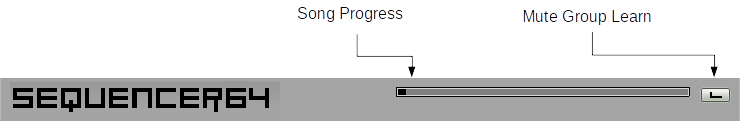
\includegraphics[scale=0.75]{pattern-window-top-panel-items.png}
   \caption{Patterns Panel, Top Panel Items}
   \label{fig:pattern_window_top_panel_items}
\end{figure}

   \begin{enumber}
      \item \textbf{Song Progress}
      \item \textbf{Mute Group Learn}
   \end{enumber}

   \setcounter{ItemCounter}{0}      % Reset the ItemCounter for this list.

   \itempar{Song Progress}{pattern!progress}
   \index{song!progress}
   \index{song!"main time"}
   The \textbf{Song Progress} bar is also known as the "main time" bar.
   This bar shows a number of small black cursors ("pills") that show the
   progress of the song through the various patterns.  For short patterns,
   the progress is fast.  For patterns that last longer, the progress is
   slow.  The whole field flashes in time with the beat.
   This field shows that something is going on.  It can also indicate
   the relative lengths of the various patterns.
 
   Note that the individual pattern boxes in the main panel, for
   patterns that are not empty, have their own
   moving progress cursor, a tall thin line in each box.

   \itempar{Mute Group Learn}{pattern!mute group learn}
   \index{"L" button}
   This button is also known as the "L" button.
   Click this button, and then press a mute-group key
   to store the mute-state of the patterns with in that key.

   See the \textbf{File / Options / Keyboard} menu entry to bring up the
   dialog showing the available mute-group keys and the corresponding
   hot-key for the "L" button.

   Group-learn is a modifier key to be pressed \textsl{together}
   with the toggle key, and the group on/off keys are there to enable/disable
   the whole feature, \textsl{not} to toggle group states.

   To set up the mute groups, press the 'L' button, and then press a key on
   the keyboard to 'learn' or 'save' the preset. Looking at the list of keys
   assigned for these mute groups (in \textbf{File / Options / Keyboard}),
   the first bank of keys are "!", "'", "?", etc., and the second bank are
   "Q", "W" "E", etc.  When you ask the program to 'learn' the key, one can't
   use the Shift key, so (on Windows at least) one cannot use the "!" or
   other symbol keys.  Similarly, make sure Caps Lock is off before starting
   the 'learn' process (as it won't recognise "q", only "Q").

   Once that works, one can configure the MIDI settings in similar ways
   by assigning MIDI commands to toggle loops, using 
   \index{rc file}
   the 'on' option in the "rc" file.
   See \sectionref{subsec:seq64_rc_file_midi_control}.

   \index{group!toggle}
	One can toggle the playing status of up to 32 previously
	defined mute/unmute patterns (groups) in the active screen
	set, similar to hardware sequencers.
   One can mute-unmute (according to the group definition) all loops in the
   playing screen set, which is the only one that can have sequences playing
   (like a live sequencer).

	This toggling is done either by one of the \textsl{group toggle} keys
	or by a MIDI controller, both assigned in the
   \index{rc file}
   \texttt{~/.config/sequencer64/sequencer64.rc} or \texttt{~/.seq24rc} files.

	A mute/unmute pattern (group) is stored by holding a
   \index{group!learn}
   \textsl{group learn} key (\texttt{Insert} by default) while pressing the
   corresponding \textsl{group toggle} key.
	There are also keys assigned to turn on/off the group functionality.

   Remember that groups work with the playing screen set only.
   One must change the screenset and give it the command to make it the
   playing one
   \index{keys!Home}
   (some set the Home key for this purpose).
   \index{rc file}
   Everything is configurable in the "rc" file.

\subsection{Patterns / Main Panel}
\label{subsec:seq64_patterns_panel_main}

   The main panel of the Patterns window provides a grid of empty boxes,
   each box delimited by brace-like lines at left and right.
   Each filled box represents a loop or pattern.
   One sees only 32 loops at a time in the main panel (but many more than
   32 loops can be supported by \textsl{Sequencer64}).
   \index{screen set}
   This group of 32 loops is called a "screen set", as discussed in
   \sectionref{subsubsec:concepts_terms_screen_set}.
   One can switch between sets by using the
   \index{keys![}
   \texttt{[} and
   \index{keys!]}
   \texttt{]} keys on the keyboard, or by using
   the spin-widget-driven, labelled \textbf{Set} interface item, or
   \index{keys!Home}
   by hitting the (default) Home key to make it the playing screenset.
   There are a total of 32 sets, for a total of 1024 loops/patterns. 
   Only one screen set can be playing at a time, according to other notes we
   have found.

\begin{figure}[H]
   \centering 
   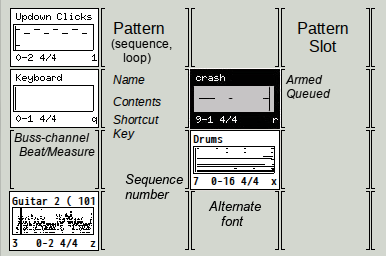
\includegraphics[scale=0.75]{pattern-window-main-panel-items.png}
   \caption{Patterns Panel, Main Panel Items}
   \label{fig:pattern_window_main_panel_items}
\end{figure}

   The individual items annoted in this figure are described in
   \sectionref{subsubsec:seq64_patterns_pattern_filled}, in more detail.

   \begin{enumber}
      \item \textbf{Pattern Slot}
      \item \textbf{Pattern}
   \end{enumber}

\subsubsection{Pattern Slot}
\label{subsubsec:seq64_patterns_pattern_slot}

   \index{pattern!slot}
   An empty box is a slot for a pattern.
   \index{pattern!right click}
   \index{slot!empty slot right-click}
   By right-clicking on an empty box one brings up a menu to create
   a new loop, as well as some other operations:

\begin{figure}[H]
   \centering 
   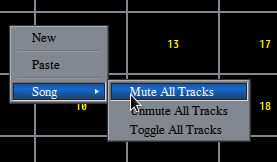
\includegraphics[scale=0.75]{pattern/pattern-empty-right-click-menu.png}
   \caption{Empty Pattern, Right-Click Menu}
   \label{fig:pattern_window_empty_right_click}
\end{figure}

   \begin{enumber}
      \item \textbf{New}
      \item \textbf{Paste}
      \item \textbf{Song / Mute All Tracks}
   \end{enumber}

   \setcounter{ItemCounter}{0}      % Reset the ItemCounter for this list.

   \itempar{New}{pattern!new}
   Creates a new loop or pattern.
   Clicking this menu entry fills in the empty box with an untitled
   pattern, and brings up the Pattern Editor
   so that one can fill in the new pattern.

   \textbf{New:}
   In addition to right-clicking and selecting \textbf{New}, the user
   \index{new!empty slot ctrl-left-click}
   can Ctrl-left-click on the empty slot, or
   \index{new!empty slot double-click}
   double-click on the empty slot, to bring up a new instance of the sequence
   editor.  For the double-click, the effect can be a bit confusing at first,
   because it currently also toggles the arming/mute status of the slot
   twice (leaving it as it was), as well.  For now, get used to it.

   \itempar{Paste}{pattern!paste}
   Pastes a loop or pattern that was previously copied.

   \itempar{Song / Mute All Tracks}{pattern!mute all}
   This item is the one item in the \textbf{Song} context menu;
   it mutes all tracks (or loops/patterns).
   It works when one has opened the Song Editor window
   and started playing in playback
   mode by starting play using that window.

   So, let us assume the song is running in playback mode.  The patterns that
   are active (unmuted) in by that playback window are shown with a black
   background in the main patterns window.  If one right clicks on a pattern
   cell and selects \textbf{Song / Mute All Tracks}, all those patterns
   will become white and be silenced.  Eventually, the Song Editor window
   catches up and shows the "M" activated for all tracks.
   
\subsubsection{Pattern}
\label{subsubsec:seq64_patterns_pattern_filled}

   A filled pattern slot is referred to informally as a pattern.
   A pattern is shown in the Pattern windows as a filled box with the
   following items of information in it.
   Examine \figureref{fig:pattern_window_main_panel_items}; it shows
   these items annotated for clarity.

   \begin{itemize}
      \item \textbf{Name}.
         \index{pattern!name}
         This line contains the name or title of the pattern, to help
         reference it when juggling a number of patters.
      \item \textbf{Contents}.
         \index{pattern!contents}
         The contents of the pattern provide a fairly detailed and
         distinguishable representation of the notes or events in the
         pattern.  Also, when the song is playing, a vertical bar cursor
         tracks the position of the playback of the pattern or loop; it
         returns to the beginning of the box every time that pattern starts
         over again.
         \textbf{New:}
         \index{new!empty pattern}
         With \textsl{Sequencer64}, an imported empty pattern will no longer
         needlessly scroll.
         However, if a pattern has even a single event (say, a program change),
         it will scroll.
         \textbf{TODO:}
         \index{todo:one-shot pattern}
         It might be good to have some patterns marked as one-shot patterns.
         They play once at the start of playback, and that is it.
         They could be marked with a cyan background.
      \item \textbf{Bus-Channel}.
         \index{pattern!bus-channel}
         This pair of numbers shows the the MIDI buss number, a dash, and
         the MIDI channel number.
         For example, "0-2" means MIDI buss 0, channel 2.
      \item \textbf{Beat}.
         \index{pattern!beat}
         This pair of numbers is the standard time-signature of the pattern,
         such as "4/4" or "3/4".  The first number is the beats-per-measure,
         and the second is the size of the beat, here, a quarter note.
      \item \textbf{Shortcut Key}.
         If the display of shortcut keys is enabled (see
         \sectionref{paragraph:seq64_menu_file_options_keyboard}),
         then the key noted in the lower-right corner of the pattern can be
         pressed to toggle the mute/unmute status of that pattern.
         This action is an alternative to left-clicking on the pattern.
      \item \textbf{Progress Cursor}.
         At the left of each box is a vertical line, waiting for playback to
         start so that it can move through the pattern, again and again.
      \item \textbf{Armed}.
         See \figureref{fig:pattern_window_main_panel_items}; it shows a black
         and grey pattern.  The black color indicates that the pattern is armed
         (unmuted), and will play if playback is initiated in the pattern
         window
         \index{live mode}
         (i.e. "live mode").
      \item \textbf{Queued}.
         That same pattern also shows that it is queued, which means that it
         will start playing when the pattern next begins again.
      \item \textbf{Alternate font}.
         Later builds of \textsl{Sequencer64} are now built with a new font.
         See \figureref{fig:pattern_window_main_panel_items}.  It shows the new
         font. 
         The old font can be selected in the "user" configuration file, and is
         also selected automatically if \textsl{Sequencer64} is run in the
         \textsl{legacy} mode.
      \item \textbf{Sequence number}.
         Later builds of \textsl{Sequencer64} are now built with the option to
         also show the sequence number in the pattern box, if the "show
         sequence numbers" option is on.
         This option can be set in the "user" configuration file.
         See \figureref{fig:pattern_window_main_panel_items}.  It shows an
         example of the sequence number, using the new font.
   \end{itemize}

   \index{pattern!left click}
   Left-clicking on an filled pattern box will toggle the status of the
   pattern between muted (white background) and unmuted (black background).
   If the song is playing via the main window, toggling this status makes
   the pattern stop playing or start playing.  Note that the armed status
   can also be toggled using hot-keys.

   Also note that, if the Song Editor is the active window and was used to
   start the playback, the pattern boxes will toggle between the muted/unmuted
   states as the music plays, and the pattern is active or inactive at the
   point of playback.  (The Song Editor acts as a list of triggers).

   \index{pattern!right click}
   By right-clicking on an already-filled box, one brings up a menu
   to allow one to edit a existing one, or perform a few other actions
   specified in the context menu.  Here is that menu:

\begin{figure}[H]
   \centering 
   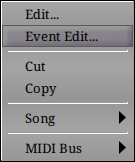
\includegraphics[scale=0.75]{pattern/pattern-right-click-menu.png}
   \caption{Existing Pattern, Right-Click Menu}
   \label{fig:pattern_window_right_click}
\end{figure}

   Here one can choose to edit the pattern, cut and copy the pattern,
   set the MIDI bus/channel, and more.
   One can also clear all performance data for the pattern.
   
   \begin{enumber}
      \item \textbf{Edit...}
      \item \textbf{Cut}
      \item \textbf{Copy}
      \item \textbf{Song/}
      \item \textbf{Midi Bus/}
   \end{enumber}

   \setcounter{ItemCounter}{0}      % Reset the ItemCounter for this list.

   \itempar{Edit}{pattern!edit}
   Edits an existing loop or pattern.
   Clicking this menu entry brings up the Pattern Editor
   so that one can modify the existing pattern.
   See \figureref{fig:pattern_edit_window}.

   \textbf{New:}
   In addition to right-clicking and selecting \textbf{Edit...}, the user
   \index{new!pattern ctrl-left-click}
   can Ctrl-left-click on the empty slot, or
   \index{new!empty slot double-click}
   double-click on the empty slot, to bring up the sequence
   editor.  For the double-click, the effect can be a bit confusing at first,
   because it currently also toggles the arming/mute status of the slot
   twice (leaving it as it was), as well.  For now, get used to it.

   \itempar{Cut}{pattern!cut}
   Deletes and copies an existing loop or pattern.
   Note than one can also drag-and-drop a pattern into another cell.
   \textbf{Bug:}
   \index{bugs!pattern cut not dirty}
   Allow this operation works, it does not cause the user to be prompted if the
   application is exited.

   \itempar{Copy}{pattern!copy}
   Copies an existing loop or pattern.
   The pattern can then be pasted elsewhere in the Patterns panel.
   See \sectionref{subsubsec:seq64_patterns_pattern_slot}.

   \itempar{Song}{pattern!song}
   Clicking this menu entry brings up a small popup menu:

\begin{figure}[H]
   \centering 
   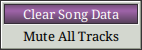
\includegraphics[scale=0.75]{pattern/pattern-menu-song.png}
   \caption{Existing Pattern, Right-Click Menu, Song}
   \label{fig:pattern_window_right_click_song}
\end{figure}

   \begin{enumber}
      \item \textbf{Clear Song Data}
      \item \textbf{Mute All Tracks}
   \end{enumber}

   \setcounter{ItemCounter}{0}      % Reset the ItemCounter for this list.

   \itempar{Clear Song Data}{pattern!clear song data}
   Selecting this filled-box right-click menu item causes that box's
   loop/pattern to be removed from the song.  This means
   that it disappears from the Song Editor window, and so will not
   be played when the song plays.

   \itempar{Mute All Tracks}{pattern!mute all tracks}
   Selecting this filled-box right-click menu item causes
   the tracks in the Song Editor to be muted.  Sometime it takes a few seconds
   for the user-interfaces to show this big change.

   \itempar{Midi Bus}{pattern!midi bus}
   Selecting this filled-box right-click menu item brings up a list
   of the 16 MIDI output busses that \textsl{Sequencer64} supports:

\begin{figure}[H]
   \centering 
   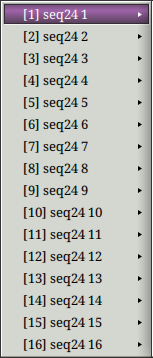
\includegraphics[scale=0.75]{pattern/pattern-menu-midi-bus.png}
   \caption{Existing Pattern, Right-Click Menu, MIDI Output Busses}
   \label{fig:pattern_window_right_click_midi_bus}
\end{figure}

   \textbf{New:}
   \index{new!--bus option}
   Note that another way of specifying the busses is to supply the
   new \texttt{--buss n} option.  This option is currently available
   only from the command line.  It causes \textsl{every} pattern in the MIDI
   file to be allocated to that buss number when loaded.  This option is
   meant for convenience or testing.  If you save the file, it will now
   have that buss number as part of each track's data.

   For each of these buss items, another pop-up menu allows one
   to specify the MIDI output channel for that buss:

\begin{figure}[H]
   \centering 
   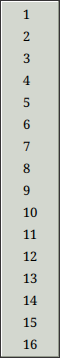
\includegraphics[scale=0.75]{pattern/pattern-menu-midi-bus-numbers.png}
   \caption{Existing Pattern, Right-Click Menu, MIDI Bus Ports}
   \label{fig:pattern_window_right_click_midi_bus_numbers}
\end{figure}

\subsubsection{Pattern Keys and Click}
\label{subsubsec:seq64_patterns_pattern_keys_and_clicks}

   This section recapitulates all the clicks and keys that perform actions
   in the Pattern windows.  Some additional clicks and keys are noted here
   as well.

\paragraph{Pattern Keys}
\label{paragraph:seq64_patterns_pattern_keys}

   Each pattern in the patterns panel can have a hot-key associated with it.
   \index{keys!hot-keys}

   \index{keys!pattern toggles}
   For each pattern, hitting its assigned keyboard key will
   also toggle its status between muted/unmuted (armed/unarmed).
   Below is the default grid that is
   mapped to the loops/patterns on the screen set.
   This grid can be changed in the Keyboard options tab, and is
   saved in the \textsl{keyboard-control} section of the
   \index{rc file}
   "rc" file.

   \begin{verbatim}
     [ 1   ][ 2   ][ 3   ][ 4   ][ 5   ][ 6   ][ 7   ][ 8   ]
     [ q   ][ w   ][ e   ][ r   ][ t   ][ y   ][ u   ][ i   ]
     [ a   ][ s   ][ d   ][ f   ][ g   ][ h   ][ j   ][ k   ]
     [ z   ][ x   ][ c   ][ v   ][ b   ][ n   ][ m   ][ ,   ]
   \end{verbatim}

   These characters are shown in the lower right corner of each
   pattern, as an aid to memory.

   These hot-keys can be modified

   \index{keys![}
   \index{keys!decrement set}
   The \texttt{[} and
   \index{keys!]}
   \index{keys!increment set}
   \texttt{]} keys on the keyboard
   switch between sets, either decrementing or incrementing the set number.

   The left and right Alt keys are, by default, set up in the
   \textbf{File / Options / Keyboard / Snapshot 1} and
   \textbf{Snapshot 2} fields to be used as "snapshot" keys.

   When one of these snapshot keys is pressed, the state of the patterns
   (which ones are armed versus unarmed) is instantly saved.  While the
   snapshot key is pressed, on can then change the state of the patterns to
   change how the song plays back.  When the snapshot key is released, the
   original saved state of the patterns is restored.

   \index{keys!alt}
   Holding \texttt{Alt} will save the state of playing patterns and restore
   them when \texttt{Alt} is lifted.

   The handling of \texttt{Alt} is generally taken over by the window
   manager, so there could be a need to change these items to some other
   keys.

%  \index{keys!left ctrl alt}
%  Holding \texttt{Left Ctrl} and \texttt{Alt} at the same time will enable
%  one to flip over to new patterns briefly and then flip right back upon
%  lifting \texttt{Alt}.  Not yet sure exactly what this means.

   \index{keys!right ctrl}
   \index{keys!queue}
   \index{queue!temporary}
	Holding \texttt{Right Ctrl} will queue a on/off toggle for a 
	sequence when the loop ends. This is the "queue" functionality.
   This means that the change in state of the pattern will not take hold
   immediately, but will kick in when the pattern restarts.

   This pending state is indicated by coloring the central box of the
   pattern grey, as shown in the following figure.

   Queue also works for mute/unmute patterns (groups). In this case every
   sequence will toggle its status after its individual loop end.

\begin{figure}[H]
   \centering 
   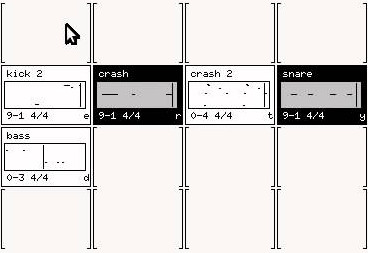
\includegraphics[scale=0.75]{pattern/seq24-queueing-coloration.jpg}
   \caption{Pattern Coloration when Queued}
   \label{fig:seq64_queueing_coloration}
\end{figure}

   Queue also works for mute/unmute 
	patterns (groups); in this case every sequence will toggle 
	its status after its individual loop end. 

   Of course, the Ctrl key is used to manage the GUI (e.g. Ctrl-q will
   unceremoniously quit the application), so one will usually want to change
   this key to something else in the
   \textbf{File / Options / Keyboard / Queue} field.
   The Super key (i.e. the Mod4 or Windows key) is a good candidate to
   replace the right Ctrl key, unless one has (like the author) configured
   the window manager to use the Super key modifier to manipulate windows
   and applications \textsl{(laughter ensues)}.

   \index{keys!replace}
   Note that there is also a "replace" key, which is the left Ctrl key by
   default.  Replacement is a form of muting/unmuting.  When the "replace"
   key is pressed while click a sequence, that sequence is unmuted, and all
   of the other sequences are muted.

   \index{keys!backslash}
   \index{keys!keep queue}
   \index{queue!permanent}
   \index{queue!keep queue}
	Pressing the "keep queue" key (by default, the backslash key)
   \index{rc file}
   assigned in the "rc" file.
	activates permanent queue mode until you use the temporary 
	queue function again pressing \texttt{Right Ctrl}. 

   This key can be changed in the
   \textbf{File / Options / Keyboard / Keep queue} field.

   There are more keys defined in the \textbf{Keyboard} dialog, and it is
   worth figuring out what they do, if not documented here.
   For a couple of short, but good, tutorials about using arming, queueing,
   and snapshots, see references \cite{wootangent1}
   and \cite{wootangent2}.

\paragraph{Pattern Clicks}
\label{paragraph:seq64_patterns_pattern_Clicks}

   \index{pattern!left click}
   \index{pattern!mute toggle}
   Left-clicking on a pattern-filled box will change its state
   \index{pattern!mute}
   \index{pattern!unmute}
   from muted (white background) to playing (black background) when
   the sequencer is running.

   \index{pattern!left ctrl left click}
   \index{keys!left ctrl}
   Holding down \texttt{Left Ctrl} while selecting a pattern
   with a left click will mute all other patterns and turn on the selected
   pattern.

   \index{pattern!left click-drag}
   By clicking and holding the left mouse button on a pattern,
   one can drag it to a new location on the grid.  The box
   will disappear while dragged, and reappear in the new location when
   dropped.  However, note that a pattern cannot be dragged if its
   Pattern Editor window is open.

   \index{pattern!right click}
   Right-clicking a pattern will bring up the appropriate context menus, as
   discussed earlier, depending on whether the pattern box is empty or
   filled.

   \index{pattern!middle click}
   Middle-click does nothing when the mouse rests inside a pattern box.

\subsection{Patterns / Bottom Panel}
\label{subsec:seq64_patterns_panel_bottom}

   The bottom panel of the Patterns window provides way to control the
   overall playback of the song.

\begin{figure}[H]
   \centering 
   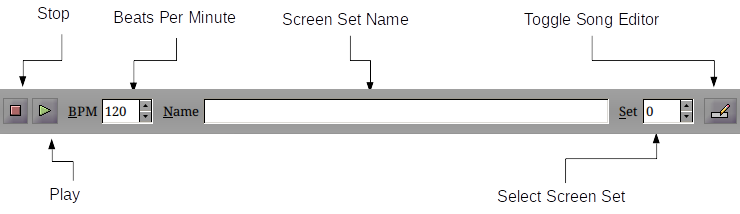
\includegraphics[scale=0.75]{pattern-window-bottom-panel-items.png}
   \caption{Patterns Panel, Bottom Panel Items}
   \label{fig:pattern_window_bottom_panel_items}
\end{figure}

   \begin{enumber}
      \item \textbf{Stop}
      \item \textbf{Play}
      \item \textbf{bpm}
      \item \textbf{Name}
      \item \textbf{Set}
      \item \textbf{Toggle Song Editor}
   \end{enumber}

   \setcounter{ItemCounter}{0}      % Reset the ItemCounter for this list.

   \itempar{Stop}{pattern!stop}
   The red squarebutton stops the playback of the song and all its patterns.
   It is not clear if it also sends MIDI Off messages on all notes.
   \index{keys!esc (stop)}
   The keystroke for stopping playback is the \texttt{Escape} character.
   It can be changed to \texttt{Space}, so that the space-bar then becomes a
   playback toggle key.

   \itempar{Play}{pattern!Play}
   The green triangular button starts the playback of the whole song.
   \index{keys!space (play)}
   The keystroke for starting playback is the \texttt{Space} character.

   \itempar{bpm}{pattern!bpm}
   The spin widget adjusts the "Beats Per Minute" or BPM value.  The
   range of this field is from 20 bpm to 500 bpm, with a default value of
   120 bpm.
   Although this field looks editable, it is not.  Most keystrokes
   that are entered actually toggle one of the pattern boxes.
   However, the following keys can also modify the BPM in small increments:
   \index{keys!semicolon} The \texttt{semicolon} reduces the BPM;
   \index{keys!apostrophe} The \texttt{apostrophe} increases the BPM.

   \itempar{Name}{pattern!set name}
   Each of the 32 available screen sets can be given a name by entering it
   into this field.

   \textbf{Bug:}
   \index{bugs!set name has side-effect}
   While one is typing in the name of the set in this field, the keystrokes
   will affect the panel window, causing playback to start and pattern
   boxes to be toggled!

   \itempar{Set}{pattern!set number}
   This spin widget selects the current screen set.  The values in this
   field range from 0 to 31, and default to 0.
   Although this field looks editable, it is not.

   \textbf{Bug:}
   \index{bugs!set number has side-effect}
   While one is typing in the number of the set in this field, the keystrokes
   will affect the panel window as well.

   \itempar{Toggle Song Editor}{pattern!toggle song editor}
   Pressing this button toggles the presence on-screen of the Song
   Editor.

%-------------------------------------------------------------------------------
% vim: ts=3 sw=3 et ft=tex
%-------------------------------------------------------------------------------
